\chapter{Experimental Setup}
\label{chapter:setup}

This work evaluates the proposed algorithms for image and text data. This chapter describes the used datasets and the evaluation methods.

\section{Datasets}
\label{chapter:datasets}

\subsection{Synthetic Data}

To motivate our approach, we manually created a dataset containing disks and rings as shown in figure \ref{fig:disksrings}. In this case, we know that single linkage performs well clustering the two rings, however it might be problematic to cluster the disks. On the other hand, complete linkage is expected to cluster the disks very well, but it might contact the two rings earlier than wanted. This data motivates our approach of interpolating between different linkage strategies, however the data is not natural and real-world datasets are very likely to have a different structure. 

\begin{figure}[h]
    \centering
    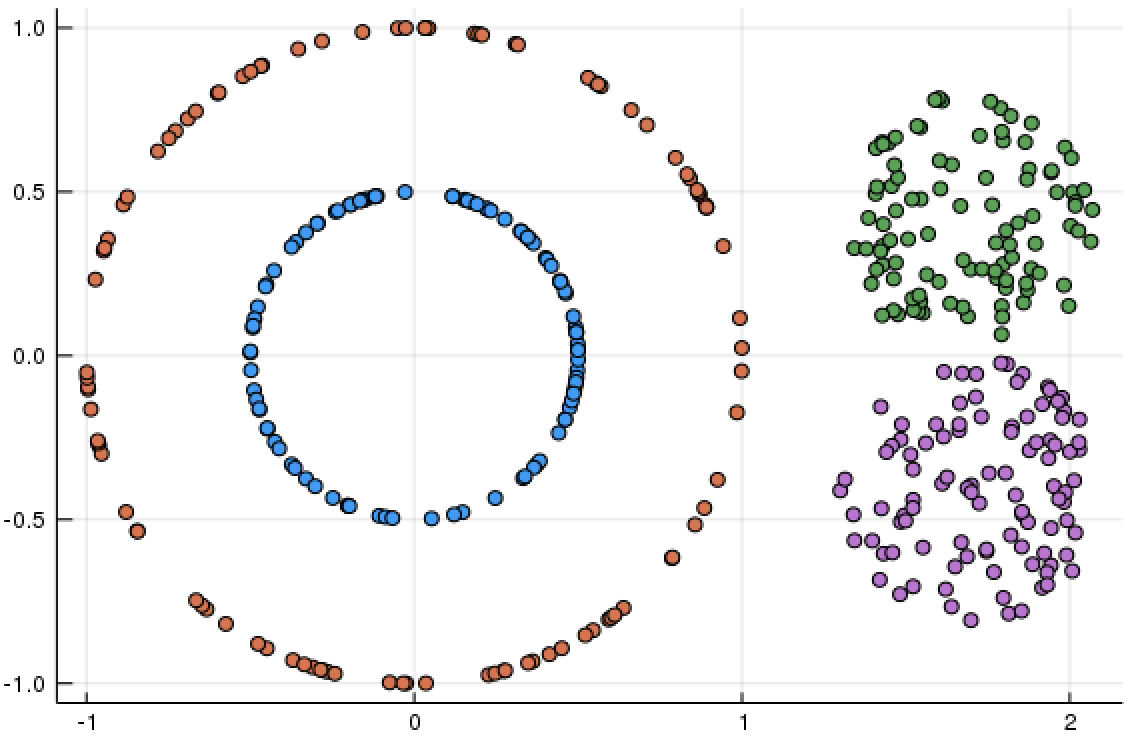
\includegraphics[width=0.7\textwidth]{images/RingsDisks}
    \caption{We use disks and rings as a sample dataset to motivate our $\alpha$-linkage approach. The dataset contains four clusters, two disks and two rings.}
    \label{fig:disksrings}
\end{figure}

\subsection{Never Ending Language Learner data}

The Never Ending Language Learner (NELL) is a learning agent that reads the web, extracts data and verifies beliefs \cite{Mitchell:2015:NL:2886521.2886641}\cite{Mitchell:2018:NL:3210350.3191513}. NELL for example knows that "Pittsburgh" is located in "Pennsylvania". These beliefs represent different noun-phrases such as "Pittsburgh" and "Pennsylvania". The noun-phrases belong to certain categories. "Pittsburgh" is a "City" and "Pennsylvania" is a "State". These subcategories both belong to the main category "Geopolitical Location". While there are already different subcategories, the goal for a hierarchical clustering algorithm here is to extract new useful subcategories.

The used dataset, extracted web-information by NELL, contains 32 different main categories, such as "Animal", "Location" or "Person". Each of these consists of up to 250 different entities that belong to different subcategories. Exemplary entites for the category "Animal" are "Otter", "Squirrel" or "Wolf". 

This thesis shows in chapter \ref{sec:results} the learned subcategories.

\subsection{MNIST handwritten digits}

The MNIST handwritten digit database contains images of the handwritten digits from zero to nine \cite{lecun-mnisthandwrittendigit-2010}. Samples of these images are shown in figure \ref{fig:mnist} Its training set contains a total of 60,000 images, where each image is represented as a 784-dimensional vector corresponding to a greyscale image with 28x28 pixels.

\begin{figure}[h]
    \centering
    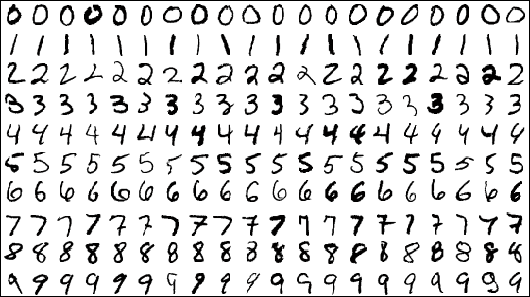
\includegraphics[width=0.7\textwidth]{images/mnist}
    \caption{The MNIST handwritten digits database contains 60,000 greyscale images of handwritten digits ranging from zero to nine. These samples show ten randomly drawn samples for each label represented as a 28x28 pixel image \cite{lecun-mnisthandwrittendigit-2010}.}
    \label{fig:mnist}
\end{figure}

The goal of clustering MNIST images is to find an unsupervised learning method that can distinguish between greyscale images. In addition, we can define various clustering tasks where we pick a subsample of the ten labels and then try to transfer the results to other subsamples. For example, we first cluster images labeled as zero, one, two, three or four and later apply the knowledge the learned gained for clustering images labeled as five, six, seven, eight or nine. Theses types of experiments allow high-level transfer learning if we define several different clustering tasks, e.g. for five different labels there are $10 \choose 5$ $= 252$ different combinations of labels.

Another obsevation that results from hierarchical clustering is the similarity of different labels, i.e. which labels are likely to get clustered together.

\subsection{CIFAR-10}

Another image dataset this thesis uses for evaluation is the CIFAR-10 dataset that contains 60,000 RGB images of ten different categories \cite{Krizhevsky2009LearningML}. Each image consists of 32x32 pixels and is thus represented as a 3072-dimensional vector (32x32x3). The categories and ten random images from each are shown in figure \ref{fig:cifar10}.

\begin{figure}[h]
    \centering
    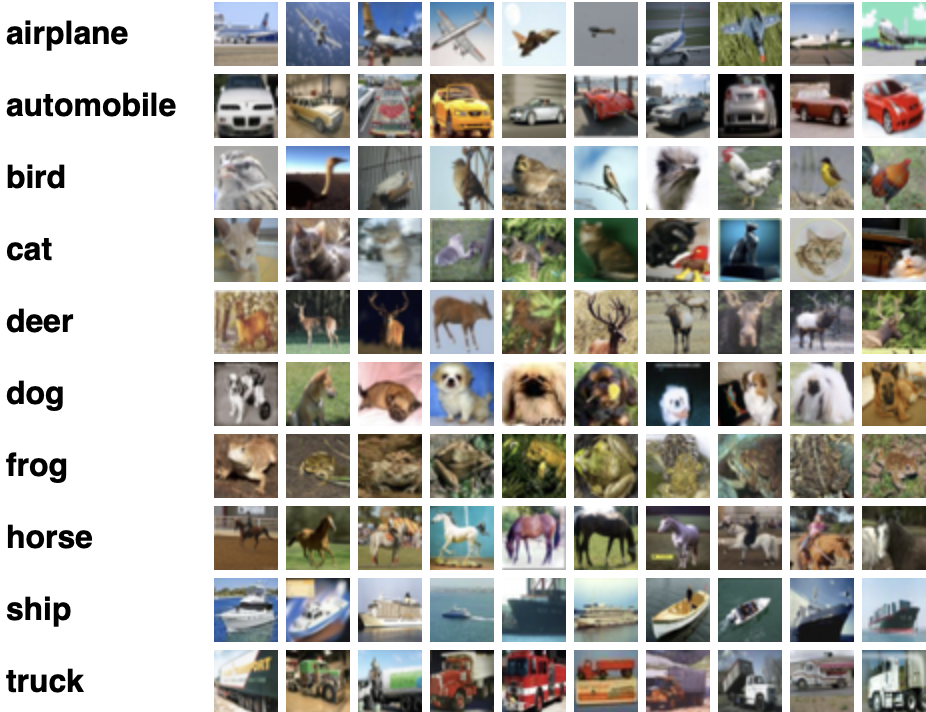
\includegraphics[width=0.7\textwidth]{images/cifar10}
    \caption{The CIFAR-10  database contains 60,000 RGB images of the ten shown different classes. These samples show ten randomly drawn samples for each label represented as a 32x32 pixel image \cite{Krizhevsky2009LearningML}.}
    \label{fig:cifar10}
\end{figure}

As the amount of images and the amount of classes is equal to the ones in the MNIST database, we can also try similar experiments. The main difference is that the images consist of RGB pixels instead of greyscale values.

\subsection{CIFAR-100}

The CIFAR-100 dataset contains similar images, but instead of 6,000 images each for 10 classes, it consists of 600 images each for 100 classes. The classes are divided into 20 superclasses each containing five subclasses. Examples of superclasses and corresponding subclasses are shown in table \ref{table:cifar100data}. 

\begin{table}[h]
    \centering
    \begin{tabular}{|l|l|}
    \hline
    superclass      & subclasses                                  \\ \hline
    aquatic mammals & beaver, dolphin, otter, seal, whale         \\
    fish            & aquarium fish, flatfish, ray, shark, trout  \\
    flowers         & orchids, poppies, roses, sunflowers, tulips \\
    people          & baby, boy, girl, man, woman                 \\ 
    reptiles        & crocodile, dinosaur, lizard, snake, turtle  \\ \hline               
    \end{tabular}
    \caption{The CIFAR-100 dataset contains 20 different superclasses, each with five different subclasses leading to 100 classes overall. The images are represented in the same way as in the CIFAR-10 dataset, i.e. by a 3072-dimensional vector \cite{Krizhevsky2009LearningML}.}
    \label{table:cifar100data}
\end{table}

Having superclasses and subclasses allows clustering between different subclasses within a superclass and also between different superclasses. This allows more experiments than for the CIFAR10 data.

\subsection{Omniglot}

The omniglot dataset contains 1623 handwritten characters from 50 different alphabets, where each character is represented by 20 different images. Each image is grayscale and represented by 105x105 pixels \cite{Lake1332}. Figure \ref{fig:omniglotcharacters} shows characters of the more well-known Latin, Greek and Hebrew alphabets that are part of the dataset.

\begin{figure}[h]
\centering
\begin{minipage}{.3\textwidth}
  \centering
  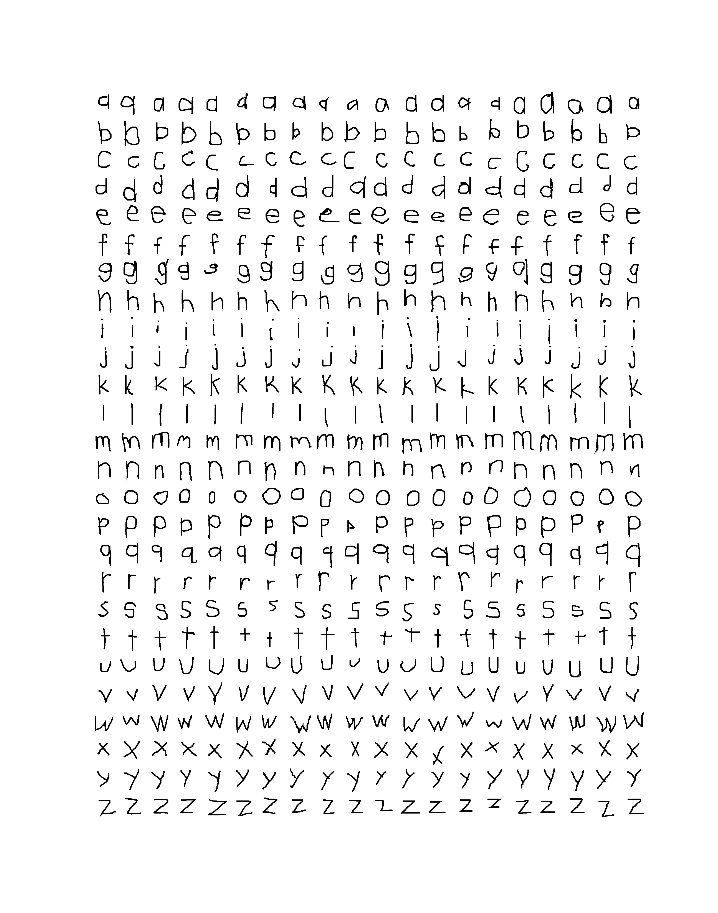
\includegraphics[width=\linewidth]{images/latin}
\end{minipage}
\begin{minipage}{.3\textwidth}
  \centering
  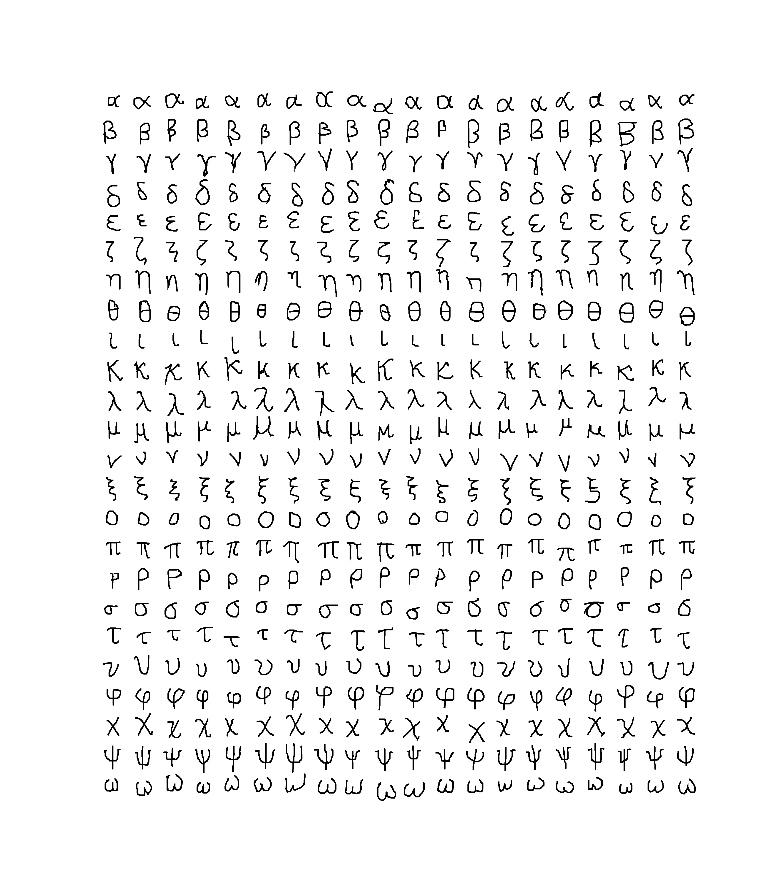
\includegraphics[width=\linewidth]{images/greek}
\end{minipage}
\begin{minipage}{.3\textwidth}
  \centering
  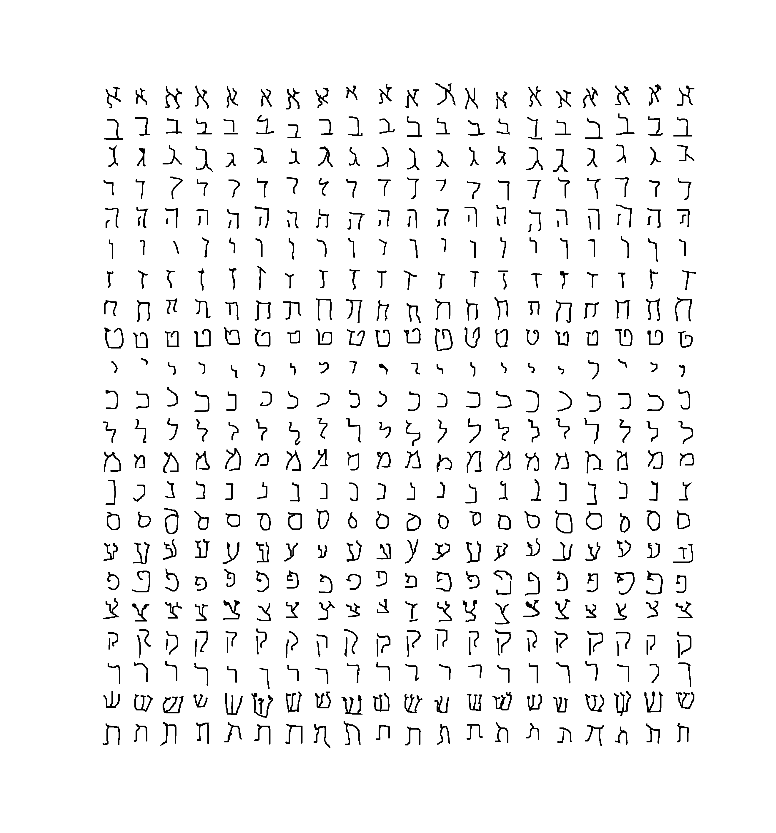
\includegraphics[width=\linewidth]{images/hebrew}
\end{minipage}
\caption{The omniglot dataset contains handwritten characters of different alphabets, such as Latin (left), Greek (middle) and Hebrew (right) \cite{Lake1332}.}
\label{fig:omniglotcharacters}
\end{figure}

The omniglot dataset is similar to the MNIST dataset as it also contains handwritten characters, however it has more different characters and less images of each of them. This allows us to run more learning tasks.

\section{Cost functions}
\label{chapter:costfunctions}

In order to evaluate the quality of a clustering, we need some kind of cost function that compares the generated clustering $C_1,...,C_k$ with the target clustering $C_1^*, ..., C_k^*$. 

\paragraph{Majority Cost.} One method to compare them is the majority distance as shown in equation \ref{eq:majoritydistance} where $n$ ist the number of sampled points.

\begin{equation}
    \begin{aligned}
        cost_{majority}(C_{1:k}, C_{1:k}^*) = \frac{1}{n} \sum_{i=1}^k \min_{j \in [m]} |C_i - C'_j|
    \end{aligned}
    \label{eq:majoritydistance}
\end{equation}

This cost function is motivated by finding corresponding clusters with the lowest distance, i.e. each generated cluster gets matched with the optimal target cluster. However two generated clusters can be matched with the same target cluster. 

\paragraph{Hamming  Cost.} This motivates the hamming distance as shown in figure \ref{eq:hammingdistance}.

\begin{equation}
    \begin{aligned}
        cost_{hamming}(C_{1:k}, C'_{1:k}) = \frac{1}{n} \min_{\sigma \in \mathbb{S}_k} \sum_{i=1}^k |C_i - C'_{\sigma_i}|
    \end{aligned}
    \label{eq:hammingdistance}
\end{equation}

However, the hamming distance consists of an assignment problem to find the optimal matching $\sigma$ between the generated clusters and the target clusters. Table \ref{table:matching} shows how such a matching can look like.

\begin{table}[h]
    \centering
    \begin{tabular}{|l | l l l l l|}
    \hline
    j\textbackslash i & 1 & 2 & 3 & 4 & 5\\ \hline
    1 & 20 & \cellcolor{blue!25}15 & 30 & 50 & 40\\
    2 & 80 & 10 & \cellcolor{blue!25}15 & 20 & 30\\
    3 & \cellcolor{blue!25}20 & 30 & 50 & 80 & 60\\
    4 & 30 & 50 & 40 & \cellcolor{blue!25}20 & 10\\
    5 & 20 & 30 & 40 & 50 & \cellcolor{blue!25}25\\ \hline
    \end{tabular}
    \caption{In order to calculate the hamming distance between two clusterings, we have to calculate the optimal mapping that results in lowest distance for these two clusterings. For random distances between clusterings $C_1^i, ..., C_k^i$ and $C_1^j, ..., C_k^j$ we can calculate the optimal mapping (blue highlighted cells) in a brute force way or more efficiently with the hungarian method \cite{kuhn1955hungarian}\cite{munkres1957algorithms}.}
    \label{table:matching}
\end{table}

While solving the assignment with a brute force strategy would result in $O(n!)$ complexity, Harold Kuhn introduced the hungarian method to solve the problem in $O(n^4)$ complexity \cite{kuhn1955hungarian}. Later on, James Munkred modified the algorithm to $O(n^3)$ complexity \cite{munkres1957algorithms}. A detailed explanation of the hungarian method is included in appendix \ref{sec:hungarian}.


\section{Parameter Advising}

Our settings average over multiple experiments and show one parameter $\alpha$ that represents the best clustering over all experiments, i.e. the algorithm automatically outputs the best result. For parameter advising, we select the top $k$ values of $\alpha$ for each experiment and calculate the clustering's cost with the best of the $k$ values of $\alpha$ \cite{deblasio2015parameter}. We select the pool of $\alpha$-values through the local optima for each experiment. The best $k$ values of $\alpha$, where $k$ is much smaller than the number of experiments, can then be calculated with an integer optimization problem. A scenario where this setup can be used is by having a domain expert, who can select the best clustering from the $k$ suggested ones.\\

More formally, we want to to find the optimal parameters $\alpha_1^*, \dots, \alpha_k^*$ such that they optimize the utility $u$ of a clustering instance $S$ and the resulting clustering tree $T(S, \alpha)$ (see equation \ref{eq:advising}). In order to calculate the parameters $\alpha_1^*, \dots, \alpha_k^*$, we first have a look at parameter advising described as facility location problem.

\begin{equation}
  \alpha_1^*, \dots, \alpha_k^*
  = \argmax_{\alpha_1, \dots, \alpha_k} \sum_{i=1}^N \max_{j \in [k]} u\bigl(S, T(S, \alpha_j)\bigr).
  \label{eq:advising}
\end{equation}

\paragraph{Facility Location Advising.} We create an integer optimization problem for a candidate set $\alpha_1, \dots, \alpha_m$ over the clustering instances $S_1, \dots, S_N$ and introduce the selection parameters $y_1, \dots, y_m \in \{0, 1\}$ that indicate whether $\alpha_j$ is used as one of the $k$ parameters. Also, we denote $x_{ij} \in \{0, 1\}$ as the auxiliary variable with the interpretation that $x_{ij} = 1$ whenever $\alpha_j$ is the best chosen parameter for problem instance $S_i$. This leads to the following optimization problem that optimizes the overall utility.

\begin{align*}
  \argmax_{x_{ij}, y_j} \qquad&\sum_{i = 1}^N \sum_{j = 1}^m x_{ij} u(S_i, T(S_i, \alpha_j)) \\
  \text{subject to} \qquad& \sum_{j=1}^m y_j = k \\
  & \text{for each $i \in [N]$, } \sum_{j=1}^m x_{ij} = 1 \\
  & \text{for each $i \in [N], j \in [M]$, } x_{ij} \leq y_j.
\end{align*}

Note that the optimization problem contains three constraints. $\sum_{j=1}^m y_j = k$ makes sure that exactly $k$ values are used, the second guarantees that we assign clustering instance to at most one parameter, and the final constraint ensures that we only assign clustering instances to selected parameters. In our experiments, we use IBM ILOG’s CPLEX to solve these integer programming problems. However, the computation of the optimal values is very complex, so we also implement a greedy strategy that calculates approximately optimal values more efficiently.

\paragraph{Greedy Parameter Advising.} In a convex space, it is very likely that an optimal value $\alpha_n^*$ will also be optimal when calculating $k = n + 1$ optimal values. Leveraging this knowledge, we can iteratively calculate the optimal values $\alpha_1, \dots, \alpha_m$ step by step, where we first calculate $\alpha_1^*$ that has the largest utility over all clustering instances $S$ and then calculate $\alpha_2^*$ that results in the highest utility combined with $\alpha_1^*$ (see equation \ref{eq:greedypa}).

\begin{equation}
\sum_{i=1}^N \max\{u(S_i, T(S_i, \alpha_1)), u(S_i, T(S_i, \alpha_2)\} 
\label{eq:greedypa}
\end{equation}

The results of the experiments with the mentioned datasets are discussed in the following section \ref{sec:results}.